% !TeX program = xelatex
\documentclass[
  convert={density=500, size=600, outext=.png}, 
  border=2pt
]{standalone}

\usepackage{fontspec}
\defaultfontfeatures{Ligatures={NoCommon,%
			NoDiscretionary,%
			NoHistoric,%
			NoRequired,%
			NoContextual}}
\setsansfont{Carlito}[%
	SmallCapsFeatures={Letters=SmallCaps},%
	SmallCapsFont={Roboto},%
	ItalicFeatures={SmallCapsFont=Roboto-Italic},%
	BoldFeatures={SmallCapsFont=Roboto-Bold},%
	BoldItalicFeatures={SmallCapsFont=Roboto-BoldItalic}%
]

\usepackage{tikz}
\usepackage{tikz-cd}
\usetikzlibrary{%
	calc,%
	arrows.meta,%
	arrows,%
	automata,%
	overlay-beamer-styles,%
	snakes,%
	shapes.arrows,%
	shapes.geometric,%
	shapes.symbols,%
	fit,%
	positioning,%
	decorations.pathreplacing,%
	backgrounds,%
}
\tikzset{
	>=Triangle,%
	nodes={align=center},%
	comp/.style={%
			draw,%
			rectangle,%
			very thick,%
			rounded corners,%
			minimum width=2.5cm,%
			minimum height=1cm,%
			fill=white},%
	input/.style={draw,%
			rectangle,%
			thick,%
			minimum width=2.5cm,%
			minimum height=1cm,%
			fill=white},%
	classnode/.style={%
			fill=cgreenlight,%
			rectangle,%
			draw,%
			inner xsep=0},%
	interfacenode/.style={%
			fill=corangelight,%
			rectangle,%
			draw,%
			inner xsep=0},%
	abstractclassnode/.style={%
			fill=cbluelight,%
			rectangle,%
			draw,%
			inner xsep=0},%
	inlinenode/.style={%
			inner xsep=.5cm,%
			minimum height=.6cm},%
}

\definecolor{reddy}{RGB}{172, 0, 51}
\definecolor{dkred}{rgb}{.6, 0, 0}
\definecolor{dkgreen}{rgb}{0, .5, 0}
\definecolor{dkblue}{rgb}{0, 0, .5}
\definecolor{cred}{RGB}{219, 68, 55}
\definecolor{credlight}{RGB}{250, 227, 225}
\definecolor{cgreen}{RGB}{3, 148, 77}
\definecolor{cgreenlight}{RGB}{209, 251, 230}
\definecolor{cblue}{RGB}{2, 119, 189}
\definecolor{cbluelight}{RGB}{208, 237, 254}
\definecolor{corange}{RGB}{173, 128, 2}
\definecolor{corangelight}{RGB}{253, 219, 123}
\newcommand{\cblue}[1]{\textcolor{cblue}{#1}}
\newcommand{\bfcblue}[1]{\textcolor{cblue}{\textbf{#1}}}
\newcommand{\cred}[1]{\textcolor{cred}{#1}}
\newcommand{\bfcred}[1]{\textcolor{cred}{\textbf{#1}}}
\newcommand{\cgreen}[1]{\textcolor{cgreen}{#1}}
\newcommand{\bfcgreen}[1]{\textcolor{cgreen}{\textbf{#1}}}
\newcommand{\corange}[1]{\textcolor{corange}{#1}}
\newcommand{\bfcorange}[1]{\textcolor{corange}{\textbf{#1}}}
\newcommand{\interfacename}[1]{\underline{\textbf{\textit{#1}}}}
\newcommand{\absclassname}[1]{\textbf{\textit{#1}}}
\newcommand{\classname}[1]{\textbf{#1}}

\usepackage{amsmath}
\usepackage{amsfonts}
\usepackage{amssymb}

\usepackage{silence}
\WarningsOff*


\begin{document}
\sffamily

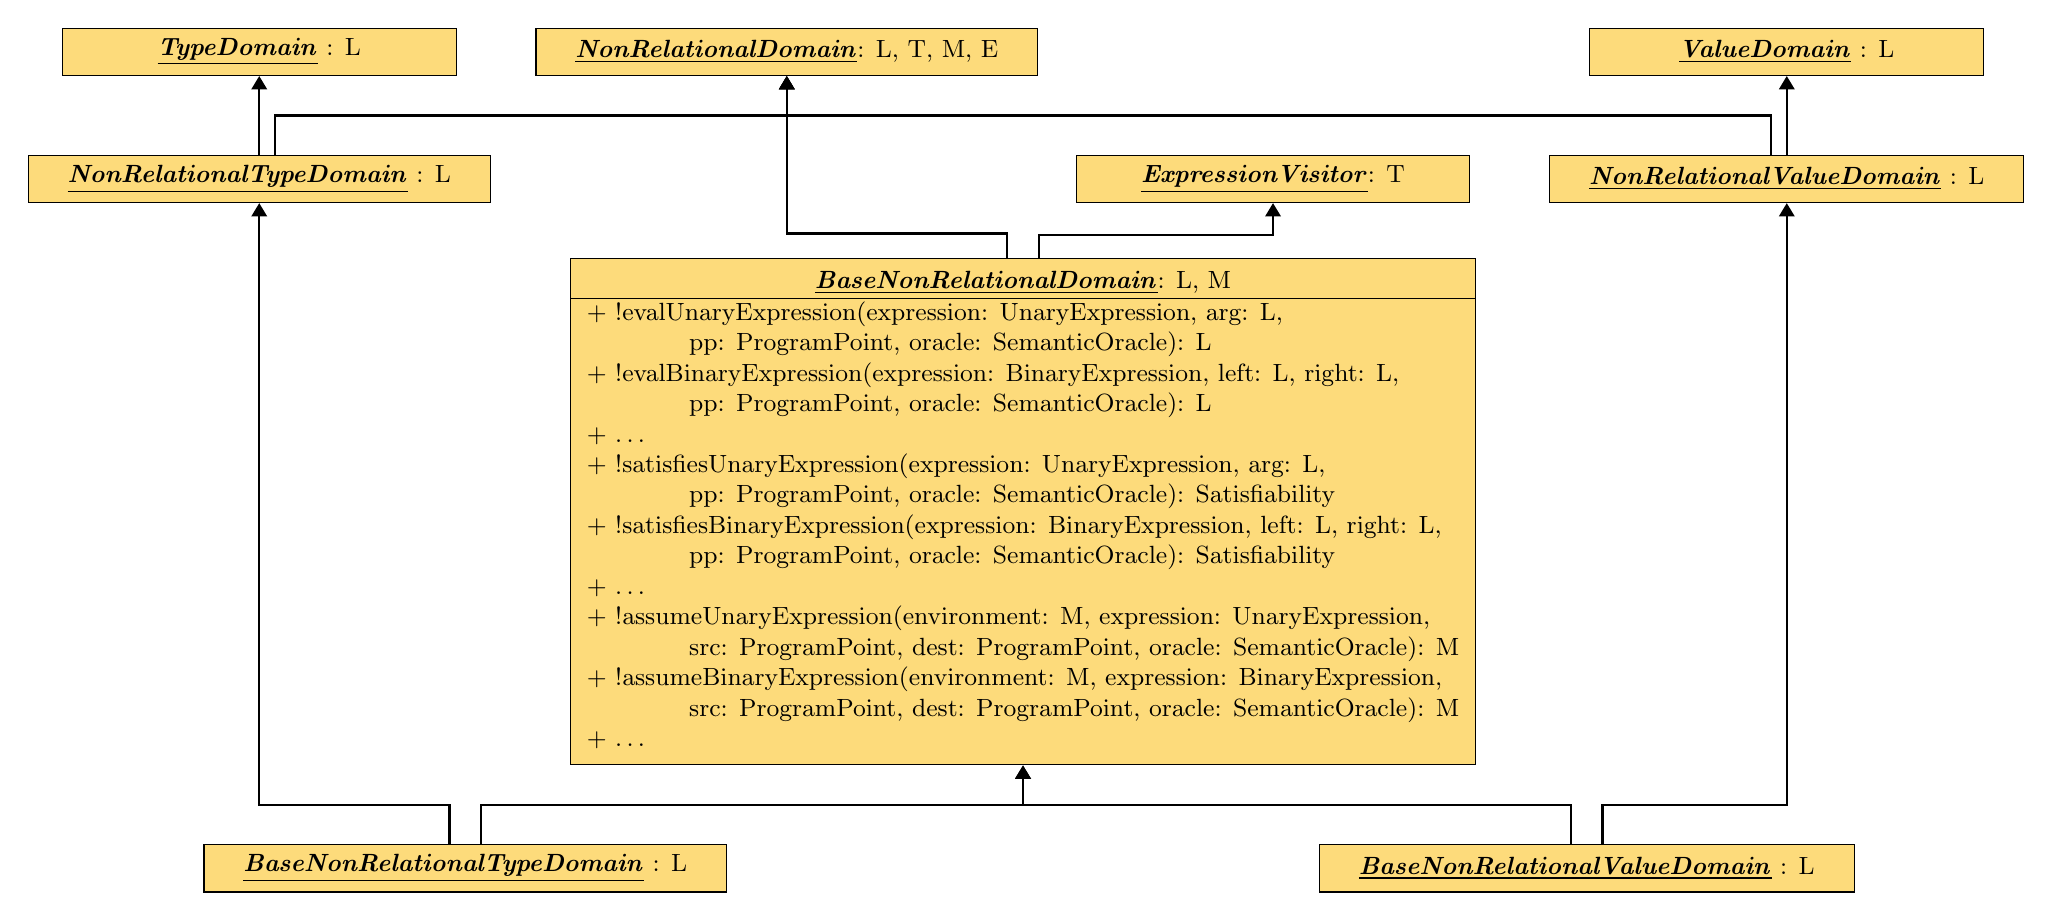
\begin{tikzpicture}[nodes={font={\small}, minimum width=5cm, minimum height=.6cm}]%
	\node[interfacenode, inlinenode] (nrd) {\interfacename{NonRelationalDomain}: L, T, M, E};
	\node[interfacenode, inlinenode] (td) [left=of nrd] {\interfacename{TypeDomain} : L};
	\node[interfacenode, inlinenode] (nrtd) [below=of td] {\interfacename{NonRelationalTypeDomain} : L};
	\node[interfacenode, inlinenode] (vd) [right=7cm of nrd] {\interfacename{ValueDomain} : L};
	\node[interfacenode, inlinenode] (nrvd) [below=of vd] {\interfacename{NonRelationalValueDomain} : L};
	\node[interfacenode, inlinenode] (ev) [left=of nrvd] {\interfacename{ExpressionVisitor}: T};

	\node[interfacenode] (bnrd) [below=of $(nrvd)!0.5!(nrtd)$] {\begin{tabular}{l}
			\multicolumn{1}{c}{\interfacename{BaseNonRelationalDomain}: L, M}               \\
			\hline
			+ !evalUnaryExpression(expression: UnaryExpression, arg: L,                     \\
			$\qquad\qquad$pp: ProgramPoint, oracle: SemanticOracle): L                      \\
			+ !evalBinaryExpression(expression: BinaryExpression, left: L, right: L,        \\
			$\qquad\qquad$pp: ProgramPoint, oracle: SemanticOracle): L                      \\
			+ $\dots$                                                                       \\
			+ !satisfiesUnaryExpression(expression: UnaryExpression, arg: L,                \\
			$\qquad\qquad$pp: ProgramPoint, oracle: SemanticOracle): Satisfiability         \\
			+ !satisfiesBinaryExpression(expression: BinaryExpression, left: L, right: L,   \\
			$\qquad\qquad$pp: ProgramPoint, oracle: SemanticOracle): Satisfiability         \\
			+ $\dots$                                                                       \\
			+ !assumeUnaryExpression(environment: M, expression: UnaryExpression,           \\
			$\qquad\qquad$src: ProgramPoint, dest: ProgramPoint, oracle: SemanticOracle): M \\
			+ !assumeBinaryExpression(environment: M, expression: BinaryExpression,         \\
			$\qquad\qquad$src: ProgramPoint, dest: ProgramPoint, oracle: SemanticOracle): M \\
			+ $\dots$                                                                       \\
		\end{tabular}};

	\node[interfacenode, inlinenode] (bnrvd) [below right=1cm and -2cm of bnrd] {\interfacename{BaseNonRelationalValueDomain} : L};
	\node[interfacenode, inlinenode] (bnrtd) [below left=1cm and -2cm of bnrd] {\interfacename{BaseNonRelationalTypeDomain} : L};

	\draw[->, thick] (nrvd) to (vd);
	\draw[->, thick] (nrtd) to (td);
	\draw[->, thick] ($(nrtd.north)+(0.2,0)$) |- ($(nrd.south)+(0,-0.5)$) to (nrd);
	\draw[->, thick] ($(nrvd.north)+(-0.2,0)$) |- ($(nrd.south)+(0,-0.5)$) to (nrd);
	\draw[->, thick] ($(bnrd.north)+(-0.2,0)$) |- ($(nrd.south)+(0,-2.0)$) to (nrd);
	\draw[->, thick] ($(bnrd.north)+(0.2,0)$) |- ($(ev.south)+(0,-0.4)$) to (ev);
	\draw[->, thick] ($(bnrvd.north)+(-0.2,0)$) |- ($(bnrd.south)+(0,-0.5)$) to (bnrd);
	\draw[->, thick] ($(bnrvd.north)+(0.2,0)$) to ($(bnrvd.north)+(0.2,0.5)$) -| (nrvd);
	\draw[->, thick] ($(bnrtd.north)+(0.2,0)$) |- ($(bnrd.south)+(0,-0.5)$) to (bnrd);
	\draw[->, thick] ($(bnrtd.north)+(-0.2,0)$) to ($(bnrtd.north)+(-0.2,0.5)$) -| (nrtd);
\end{tikzpicture}

\end{document}
